\section{Datensatz} \label{sec:data_set}

Der folgende Abschnitt soll sich mit dem verwendeten Datensatz auseinandersetzen. Dazu gehört eine Evaluation verschiedener Datensätze und die Selektion des am besten geeigneten. Des Weiteren soll auf einige Methoden eingegangen werden, die den gewählten Datensatz auf den hier vorliegenden Anwendungsfall anpassen.

Für die Erstellung eines Datensatzes existieren grundsätzlich zwei Möglichkeiten. Der erste Ansatz besteht darin, die Datensammlung selbst durchzuführen und die Daten beispielsweise von der Webseite eines Fashion-Online-Shops zu extrahieren. Diese Methode bietet einen hohen Grad an Flexibilität, ist allerdings sehr aufwendig. Die Alternative besteht darin einen bereits existierenden Datensatz zu verwenden und die Erstellung so deutlich zu vereinfachen. Aufgrund des großen zeitlichen Aufwands der ersten Variante und der Verfügbarkeit verschiedener vorgefertigter Fashion-Datensätze soll in diesem Projekt der zweite Ansatz verfolgt werden.

Dementsprechend muss aus den verfügbaren Optionen die ausgewählt werden, die den Anforderungen des Projektes am meisten genügt. Mögliche Datensätze sind Fashion Product Images Dataset \cite{FashionProduct2019}, Fashionpedia \cite{Fashionpedia2020}, Fashion-MNIST \cite{FashionMNIST2017} und Deepfashion \cite{DeepFashion2016}. Ein Vergleich der Optionen ist in Tabelle \ref{tab:compareSets} dargestellt. 

\begin{table}[H]
\centering
\resizebox{0.95\textwidth}{!}{%
\begin{tabular}{lll}
\toprule
Datensatz & Vorteile & Nachteile \\ 
\midrule
Fashion Product Images  
    & \tabitem mehr als 44.000 Bilder
    & \tabitem Nicht alle Klassen notwendig\\
    & \tabitem Vielzahl an Klassen/ Attributen
    & \tabitem i.d.R Frontalperspektive\\
    & \tabitem Ein Objekt im Zentrum
    & \tabitem Hintergrund immer weiß
    \bigskip\\
Fashionpedia            
    & \tabitem mehr als 48.000 Bilder 
    & \tabitem Mehrere Objekte pro Bild\\
    & \tabitem Vielzahl an Klassen/ Attributen
    & \tabitem Nicht alle Klassen notwendig\\
    & \tabitem Bilder aus verschiedenen Perspektiven
    &  
    \bigskip\\
Fashion-MNIST           
    & \tabitem integriert in Tensorflow-Datasets
    & \tabitem geringe Anzahl an Klassen/ Attributen\\
    & \tabitem mehr als 60.000 Bilder
    & \tabitem Schwarz-Weiß-Bilder
    \bigskip\\
Deepfashion             
    & \tabitem mehr als 800.000 Bilder         
    & \tabitem unterteilt in verschiedene Benchmarks\\ 
    & \tabitem Vielzahl an Klassen/ Attributen
    & \tabitem Benötigte Attribute nicht in allen Benchmarks\\
\bottomrule
\end{tabular}}
\caption{Vergleich verschiedener Fashion-Datensätze}
\label{tab:compareSets}
\end{table}

Aufgrund dessen, dass die Kleidung i. d. R. isoliert abgebildet wird und eine ausreichende Auswahl an Attributen existiert, soll der Fashion Product Images Datensatz verwendet werden. Fashionpedia wurde ausgeschlossen, weil zusätzlich zu der Klassifizierung noch eine Segmentierung des Bildes notwendig wäre und Fashion-MNIST aufgrund dessen, dass dieser keine befriedigende Komplexität für diesen Anwendungsfall bietet. Die Daten des In-shop Clothes Retrieval Benchmark aus Deepfashion stellen ebenfalls einen geeigneten Datensatz dar, sollen jedoch vorerst nicht verwendet werden. Allerdings soll die Möglichkeit offen gehalten werden diesen in Teilen oder komplett zusätzlich zu nutzen, um eventuelle Ungleichverteilungen auszugleichen oder die Datenmenge zu vergrößern.

Bevor der Datensatz verwendet werden kann, müssen jedoch noch einige Analysen durchgeführt werden und infolgedessen Anpassungen vorgenommen werden. Zu den Änderungen gehört die Selektion relevanter Merkmale (Accessoires werden beispielsweise nicht berücksichtigt) sowie eine sinnvolle Zusammenfassung einiger Werte (z. B. werden Jeans und Leggings Hosen zugeordnet). In Abbildung \ref{fig:evaluation} sind die Verteilungen und möglichen Ausprägungen der gewählten Klassen dargestellt.

\begin{figure}[H]
    \centering
    \begin{subfigure}[c]{0.32\linewidth}
        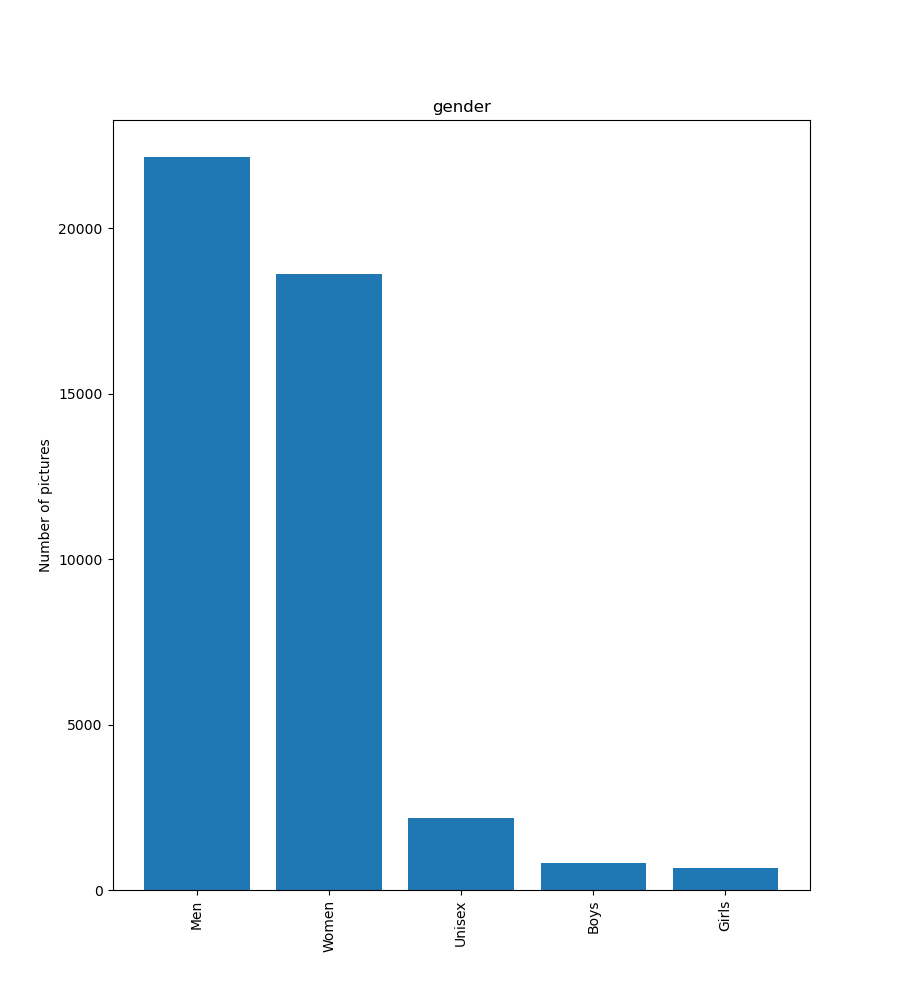
\includegraphics[width=\linewidth]{Ausarbeitung/images/gender.png}
    \end{subfigure}
    \begin{subfigure}[c]{0.32\linewidth}
        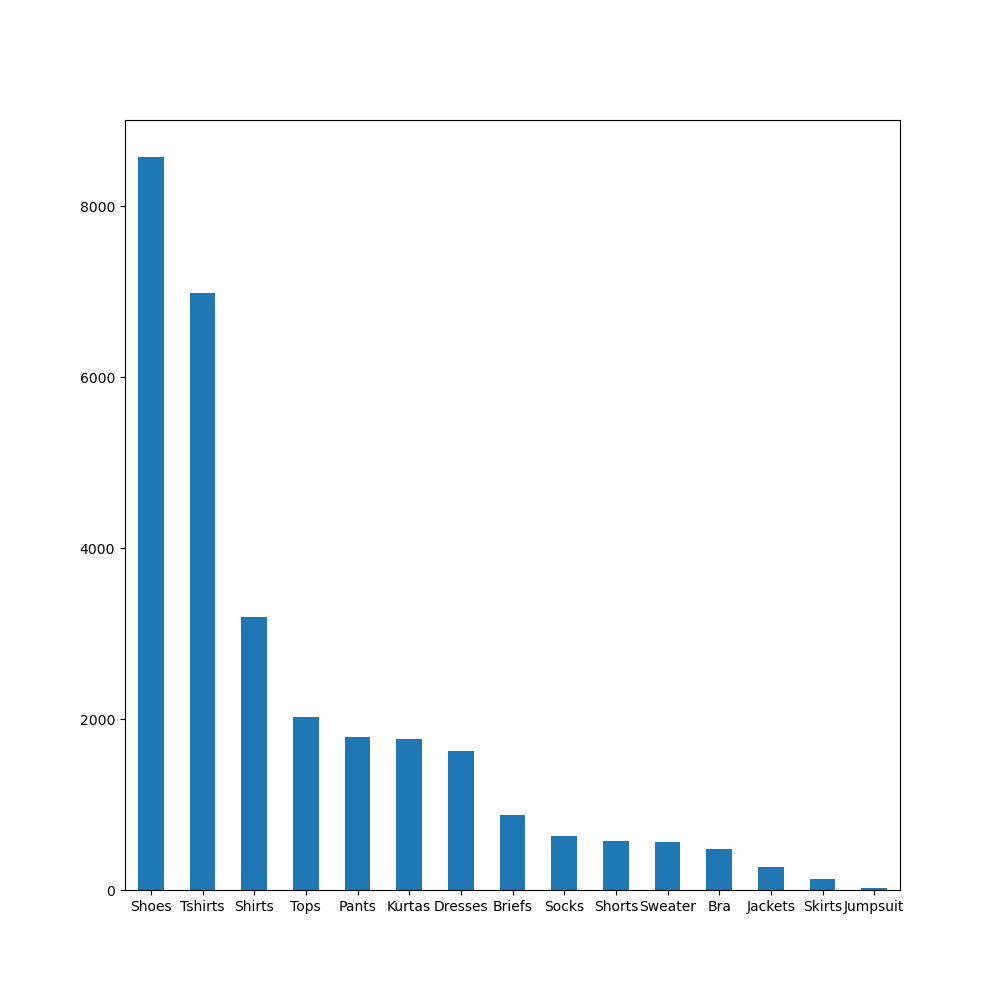
\includegraphics[width=\linewidth]{Ausarbeitung/images/articleType.png}
    \end{subfigure}
    \begin{subfigure}[c]{0.32\linewidth}
        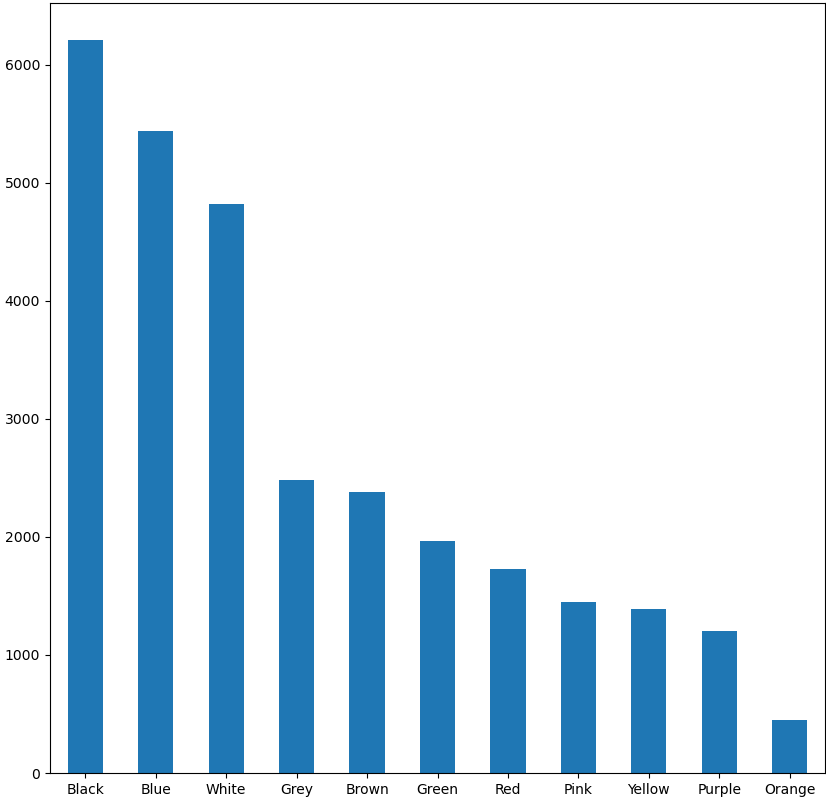
\includegraphics[width=\linewidth]{Ausarbeitung/images/baseColour.png}
    \end{subfigure}
    \caption{Verteilungen der ausgewählten Merkmale}
    \label{fig:evaluation}
\end{figure}

Für die Erstellung des verwendeten Datensatzes werden die Bilder normalisiert und augmentiert. Das heißt, sie werden auf eine einheitliche Größe gebracht und die Farbwerte auf ein Intervall von null bis eins skaliert. Bei der Erweiterung der Bilder sollen z. B. die Rotation, Helligkeit und die Spiegelung zufällig verändert werden.

Die Labels werden in Form eines Multi-Hot codierten Vektors repräsentiert. Dementsprechend steht jede eins dafür, dass eine bestimmte Ausprägung in dem Bild vorkommt. In Abbildung \ref{fig:multihot} ist das Prinzip vereinfacht dargestellt. Diese Form der Darstellung wird benötigt, damit das Modell eine Multi-Label-Klassifizierung durchführen kann.

\begin{figure}[H]
    \centering
    
\includegraphics[width=0.3\linewidth]{Ausarbeitung/images/MultiHotEncoding.png}
    \caption{Multi-Hot-Kodierung eine blauen T-Shirts für Männer}
    \label{fig:multihot}
\end{figure}

Der Datensatz soll in Traings-, Test- und Validierungsdaten aufgeteilt werden. Dabei sollen 80\% der Daten als Trainingsdaten dienen und der Rest wird gleichmäßig auf die anderen beiden Teile aufgespalten.